%implementing document formatting:
%page setup (page size, text size, page layout, chapters start on a new page).
%memoir is a form of book class that supports any kind of document.
\documentclass[fleqn,a4paper,12pt,twoside,openany]{memoir}

\usepackage{titlesec}
\usepackage{anysize}
\usepackage{enumitem}
\usepackage{graphicx}



\usepackage{pifont} % extra symbols like (v.. approved)...
\usepackage[hyphens]{url}
\usepackage{array}
\usepackage{multirow}

%\titleformat{\chapter}[display]
%{\normalfont\huge\bfseries}{\chaptertitlename\ \thechapter}{20pt}{\Huge}

% this alters "before" spacing (the second length argument) to 0

\titlespacing*{\chapter}{0pt}{-50pt}{10pt}


%setting the header and footer in that order:
\setheadfoot{28pt}{28pt} %if any problems are encountered, try changing the latter 28pt with 1cm.

%general package syntax: \usepackage[options]{package}

%setting language:
\RequirePackage[danish, english]{babel}

%this package makes it possible to treat any element as a float,
%figures and tables are by default treated as floats.
%read http://en.wikibooks.org/wiki/LaTeX/Floats,_Figures_and_Captions to specify your float.
\usepackage{float}
\usepackage{wrapfig}
\usepackage{placeins}
\usepackage{siunitx}


%this package makes it possible to make theorems and examples:
\usepackage{amsthm}
%setting the style of examples (parameters: plain, definition, remark):
%(definition is usually used for examples)
\theoremstyle{definition}
%the frist parameter is the syntax used in the document, the second is that which is printed in LaTex.
\newtheorem{example}{Example}

%making it possible to use æ, ø and å:
\usepackage[utf8]{inputenc}
%helps with word division when using æ, ø and å, and makes it ps-font rather than bmp:
\usepackage[T1]{fontenc}

%package for implementation of graphic files:
\usepackage{graphicx}

%package for captions
\usepackage[nooneline]{caption}
\usepackage{subcaption}

%%package for implementation of math:
\usepackage{amsmath, amsfonts, amssymb, float, mathtools}

%allowing use of color:
\usepackage[usenames,dvipsnames]{color}
%allowing use of more colors also in tables (see: http://en.wikibooks.org/wiki/LaTeX/Colors):
\usepackage[usenames,dvipsnames,svgnames,table]{xcolor}
\usepackage{colortbl} %Colors for tabulars
\definecolor{pwdrblue}{RGB}{140,140,140} %Color changed back!
\definecolor{darkgrey}{RGB}{180,180,180}
\definecolor{lightgrey}{RGB}{201,201,201}
\definecolor{aaublue}{RGB}{53,46,102}
\definecolor{aausub}{RGB}{154,167,180}
\definecolor{MidnightBlue}{RGB}{25, 25, 112}
\definecolor{NavyBlue}{RGB}{0, 0, 128}
\definecolor{darkgray}{gray}{0.35}
\definecolor{AleeRed}{rgb}{0.5,0,0}
\definecolor{mygreen}{rgb}{0,0.6,0}
\definecolor{mygray}{rgb}{0.5,0.5,0.5}
\definecolor{mymauve}{rgb}{0.58,0,0.82}
%hyperlinks in the tabel of contents - comment this out before the report is printed.
\usepackage{hyperref}
\hypersetup{
	bookmarks = true,  % Show 'bookmark'-frame in pdf.
	colorlinks = false, % True = colored links, False = framed links.
	citecolor = blue,  % Link color for references.
	linkcolor = blue,  % Link color in table of contents.
	urlcolor = blue,   % Link color for extern URLs.
}

%makes it possible to refer to the name of a chapter rather than just the number.
\usepackage{nameref}
\usepackage[american,cuteinductors,smartlabels]{circuitikz}
\usepackage{tikz}
\usetikzlibrary{shapes,arrows,positioning,calc}
\usetikzlibrary{calc}
\usetikzlibrary{patterns}

%package for writing program code in latex
\usepackage{listings}

\lstset{  
  backgroundcolor=\color{lightgrey},
  %escapeinside={\%*~}{*)},
  basicstyle=\small,               
  breaklines=true,                                   
  comment=[l]{//},
  commentstyle=\color{mygreen},             
  extendedchars=false,              
  frame=none,	                                   
  keywordstyle=\color{blue},
  keywordstyle=[2]\color{red},        
  language=C,                            
  numbers=left,                   
  numbersep=5pt,                   
  numberstyle=\scriptsize,                                                                          
  stringstyle=\color{mymauve},     
  tabsize=2,	             
  morekeywords=[2]{AD1PCFG,AD1CON1, AD1CSSL, AD1CON3, AD1CON2, AD1CON1SET, AD1CHS, AD1CON1CLR, AD1CHSbits, DelayUs, ADC1BUF0, CH0SA},   
 % morekeywords=[3]{CH0SA},  
 % keywordstyle=[3]\color{blue},
  identifierstyle=\ttfamily,
  %backgroundcolor=\color{white},
}

%setting references (using numbers) and supporting i.a. Chicargo-style:

\usepackage{url}

\usepackage[backend=bibtex]{biblatex}
\bibliography{bibliography/bibliography.bib}

\usepackage{verbatim} %enables /begin(comment) and /end{comment} for larger sections

%this package makes it possible include pdf pages in fx appendix;
%using  following syntax: \includepdf[pages={1}]{myfile.pdf}
\usepackage{pdfpages}

\usepackage{pbox} % used for newline in tabular

%%%MARGINER%%%
\setlrmarginsandblock{3.5cm}{2.5cm}{*}	% \setlrmarginsandblock{inner margin}{outer margin}{ratio}
\setulmarginsandblock{2.5cm}{3.0cm}{*}	% \setulmarginsandblock{top}{bottom}{ratio}
\checkandfixthelayout 			            % fixes stuff..

%Enables the use FiXme refferences. Syntax: \fixme{...}
%With "final" in stead of "draft" an error will ocure for every FiXme
%under compilation.
%\usepackage[footnote,draft,english,silent,nomargin]{fixme}

%Centering captions in tables
%\centering
%\captionsetup{justification=centering}
%\caption{bla bla bla}
\usepackage{caption}
\usepackage{pgfplotstable}
\usepackage{pgfplots}

\pgfplotsset{width=15cm,height=7cm}
\usepackage{filecontents}
\usepackage{epstopdf}
\usepackage{nomencl}
\renewcommand{\nomname}{Glossary}
\renewcommand*{\pagedeclaration}[1]{\unskip\dotfill\hyperpage{#1}}
\makenomenclature
\usepackage{makeidx}
\makeindex

%implementing macros:
%%Figure references:
\newcommand{\figref}[1]{\textbf{figur \ref{#1}}}

%Figure references after full stop/period:
\newcommand{\Figref}[1]{\textbf{Figur \ref{#1}}}

%Table references:
\newcommand{\tableref}[1]{\textbf{tabel \ref{#1}}}

%%%CHAPTERLAYOUT%%%
%setting the color of the chapter number
\definecolor{numbercolor}{gray}{0.7}
%Downloaded chapter-setup:
\newif\ifchapternonum
\makechapterstyle{jenor}{
	\setlength{\beforechapskip}{-2cm}	% Adjust space between page top and chapter title.
	\setlength{\afterchapskip}{1.5cm}	% Adjust spave between chapter title and text.
  	\renewcommand\printchaptername{}
  	\renewcommand\printchapternum{}
  	\renewcommand\printchapternonum{\chapternonumtrue}
  	\renewcommand\chaptitlefont{\fontfamily{pbk}\fontseries{db}\fontshape{n}\fontsize{25}{35}\selectfont\raggedleft}
  	\renewcommand\chapnumfont{\fontfamily{pbk}\fontseries{m}\fontshape{n}\fontsize{1in}{0in}\selectfont\color{numbercolor}}
  	\renewcommand\printchaptertitle[1]{%
    \noindent
    \ifchapternonum
    \begin{tabularx}{\textwidth}{X}
    {\let\\\newline\chaptitlefont ##1\par} 
    \end{tabularx}
    \par\vskip-2.5mm\hrule
    \else
    \begin{tabularx}{\textwidth}{Xl}
    {\parbox[b]{\linewidth}{\chaptitlefont ##1}} & \raisebox{-15pt}{\chapnumfont \thechapter}
    \end{tabularx}
    \par\vskip2mm\hrule
    \fi
  }
}
%setting chapter style:
\chapterstyle{jenor}

%depth of numbered headlines (part/chapter/section/subsection):
\setsecnumdepth{subsection}
\maxsecnumdepth{subsection}
%depth of the table of contents:
\settocdepth{section}
\parindent=0pt 

% Makes sure LaTeX does not stretch the text at page break:
\raggedbottom

\newcommand{\img}[4]{
    \begin{figure}[!ht]
    	\centering
    		\includegraphics[width=#4\textwidth]{#1}
    	\caption{\text{#2}}
    	\label{#3}
    \end{figure}
}

\newcommand{\tableimg}[3]{
    \begin{figure}[!ht]
    	\centering
    		\includegraphics[width=#3\textwidth]{#1}
    	\label{#2}
    \end{figure}
}

\newcommand{\wrapimg}[8]{
	\begin{wrapfigure}[10]{#5}{0.4\textwidth} \hspace{0pt}
	\vspace{#6}
  		\begin{center}
   			 \includegraphics[width=#4\textwidth]{#1}
  		\end{center}
  		\vspace{#7}
 		\caption{\textbf{#2}}
 	 	\label{#3}
 	 	\vspace{#8}
	\end{wrapfigure}
}

\newcommand{\sidebyimg}[4]{
	\begin{figure}[H]
		\center
		\begin{subfigure}[b]{0.48\textwidth}
			\includegraphics[width=\textwidth]{#1}
			\caption{#2}
		\end{subfigure}
		\quad
		\begin{subfigure}[b]{0.48\textwidth}
			\includegraphics[width=\textwidth]{#3}
			\caption{#4}
		\end{subfigure}
	\end{figure}
}

\newcommand{\sidebyimglabel}[8]{
	\begin{figure}[H]
		\center
		\begin{subfigure}[b]{0.48\textwidth}
			\includegraphics[width=\textwidth]{#1}
			\caption{#2}
			\label{#3}
		\end{subfigure}
		\quad
		\begin{subfigure}[b]{0.48\textwidth}
			\includegraphics[width=\textwidth]{#4}
			\caption{#5}
			\label{#6}
		\end{subfigure}
		\caption{#7}
		\label{#8}
	\end{figure}
}

\newcommand{\threesidebyimg}[9]{
	\begin{figure}[!htb]
		\minipage{0.32\textwidth}
  			\includegraphics[width=\linewidth]{#1}
  			\caption{\textbf{#2}}\label{fig:#3}
		\endminipage\hfill
		\minipage{0.32\textwidth}
  			\includegraphics[width=\linewidth]{#4}
  			\caption{\textbf{#5}}\label{fig:#6}
		\endminipage\hfill
		\minipage{0.32\textwidth}
  			\includegraphics[width=\linewidth]{#7}
  			\caption{\textbf{#8}}\label{fig:#9}
		\endminipage\hfill
	\threesidebyimgcontinued
}

\newcommand{\threesidebyimgcontinued}[1]{
	\caption{\textbf{#1}}
	\end{figure}
}

\newcommand{\blueheader}[1]{
	\cellcolor{aaublue}\textbf{\color{white}#1}
}
\begin{document}
\nomenclature{ADC}{Analog-digital conversion}
\nomenclature{PID}{Proportional-integral-derivative}
\nomenclature{THT}{Through-hole-technology}
\nomenclature{3D print}{3-Dimensional printing}
\nomenclature{PWM}{Pulse-width modulation}
\nomenclature{GUI}{Graphical User Interface}
\nomenclature{IDE}{Integrated Development Environment}
\nomenclature{MCU}{Microcontroller Unit}
\nomenclature{PCB}{Printed Circuit Board}
\nomenclature{UART}{Universal Asynchronous Receiver/Transmitter}
\renewcommand\chaptername{Chapter}
\renewcommand\contentsname{Table of Contents}
\renewcommand\figurename{Figure}
\renewcommand\tablename{Table} 

%implementing front page:
\clearpage
\thispagestyle{empty}

\begin{figure}[H]
	\raggedleft
		
\includegraphics[width=0.2\textwidth]{figures/logo-ucn.png}
\end{figure}
\vspace*{\fill} 
\begin{center}
\begin{Huge}
Fall Semester 2015\\
\vspace{5 mm}
\textbf{Line following robot}\\
\vspace{3 mm}
Group 2\\
\vspace{3 mm}
2. Semester IT-Technology
\end{Huge}
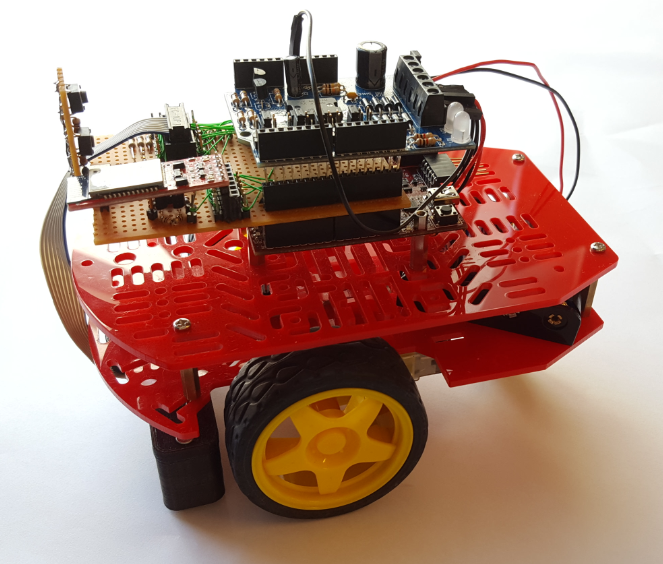
\includegraphics[width=0.7\textwidth]{figures/Forsidebil.PNG}
\end{center}
\vspace*{\fill}
\begin{center}
Group members:
 Benjamin Nielsen - Henrik Jensen - Martin Nonboe - Nikolaj Bilgrau
\end{center}
\begin{center}
Supervisor: Jesper Kristensen - Steffen Vutborg
\end{center}
\begin{center}
\line(1,0){400}
\end{center}
%clears one or two pages to make the document start on right hand side:
\cleardoublepage

%numbers the pages with Roman numeral - starts from "i":
\frontmatter

%implementing title sheet:
% Dette er LaTeX-versionen af titelbladet for tek-nat-basis-rapporter 2004 efterår
% Filen kræver:
% Universitetets logo:  aau-logo.png (for LaTeX) eller aau-logo.ps (for LaTeX)
% Synopsis: En fil ved navn synopsis.tex

% Udarbejdet af: Hans Håttel (hans@cs.auc.dk) 21. maj 2003
% Rettet af Morten Christophersen (mortench@tnb.aau.dk) 30. nov 2004(ændret til nyt design 2004 efterår)

%\documentclass[11pt]{article}
%\ifx\pdfoutput\undefined 
%\usepackage[dvips]{graphicx}
%\else
%\usepackage[pdftex]{graphicx} 
%\usepackage{type1cm} \fi
%    \usepackage[ansinew]{inputenc}
%    \usepackage{a4}

%\begin{document} 
\thispagestyle{empty}
%\begin{titlepage}
\begin{nopagebreak}
{\samepage 

\begin{tabular}{r}
\parbox{\textwidth}{  \raisebox{11mm}{
\includegraphics[height=1.5cm]{figures/logo-ucn.png}}
\hfill \hspace{2cm} \parbox{8cm}{\begin{tabular}{l} %4.90
{\small \textbf{\textcolor{MidnightBlue}{IT-technology}}}\\ 
{\small \textcolor{NavyBlue}{Sofiendalsvej 60}} \\
{\small \textcolor{NavyBlue}{9200 Aalborg SW}} \\
{\small \textcolor{NavyBlue}{\emph{http://www.ucn.dk/}}}
\end{tabular}}}
\end{tabular}

\begin{tabular}{cc}
\parbox{7cm}{
\begin{description}

\item { Title:} 

Line following robot

\end{description}

\parbox{8cm}{

\begin{description}
\item { Project Period:}\\
   2. Semester | Spring semester 2016\\
  \hspace{4cm}
\item { Projectgroup:}\\
  Group 2 
  \hspace{4cm}
\item { Medvirkende:}\\
Benjamin Nielsen\\
Henrik Jensen\\
Martin Nonboe\\
Nikolaj Bilgrau\\
\hspace{2cm}
\item { Supervisor:}\\
Jesper Kristensen\\
Steffen Vutborg
  
\end{description}
}
\begin{description}
\item { Pages: TBD} 
\item { Appendices: TBD} 
\item { Completed TBD} 
\end{description}
\vfill } &
\parbox{7cm}{
  \vspace{.15cm}
  \hfill 
  \begin{tabular}{l}
   \end{tabular}}
\end{tabular}} \vspace{1.3cm}
\centering
\\
\end{nopagebreak}
%\end{titlepage}
%\end{document}
\chapter*{Introduction}


%Læsevejledning:\\
%Kommer senere i projektforløbet.
%\\\\
Project is written by:\\
%
\phantom{Luft}\vspace{3cm}
\begin{table}[H]
	\centering
		\begin{tabular}{c c c}
			\underline{\phantom{JAERJAERJAERJAERGO}} & \phantom{cookies} & \underline{\phantom{JAERJAERJAERJAERGO}} \\
			Benjamin Nielsen			& \phantom{cookies} & Henrik Jensen		\\
			&&\\
			&&\\
			\underline{\phantom{JAERJAERJAERJAERGO}} & \phantom{cookies} & \underline{\phantom{JAERJAERJAERJAERGO}} \\
			Martin Nonboe			& \phantom{cookies} & Nikolaj Bilgrau		\\
			&&\\
						
		\end{tabular}
\end{table}

\cleardoublepage

%the '*' allows the tableofcontents be excepted from the actual table of contents.
\tableofcontents*
\newpage
\printnomenclature
\renewcommand*\listfigurename{List of Figures}
\renewcommand*\listtablename{List of Tables}

%numbers the pages with Arabic numeral - starts from 1.
\mainmatter

\chapter{Requirements specification}
The following section will list the specific requirements that have been decided to fulfil to the general requirements as shown in the project description.
\begin{enumerate}
	\item[•]Project must include light sensors
	\item[•]Implement motor control				
	\item[•]Should make use of the Pic32 MCU or the UCN board
	\item[•]Software will be written in MPLAPX
	\item[•]Must follow a line autonomously
	\item[•]The product must make use of feedback concept e.g. a PID algorithm
\item[•]A function \& performance test is to be conducted
\end{enumerate}

\chapter{Hardware section}
\section{Specification of hardware requirements}
\begin{enumerate}
	\item[•]- Main reason for not using UCN board is the limited pins available.
\\ - Project must include light sensors
\\ - Should make us of the Pic32 MCU
\\ - Autonomous operation - Feedback concept
\\ - Faster rate than UCN board, up to 80MHz.
\\ - Function testing
\\ - Performance testing

	\begin{enumerate}
		\item[-]TBD
	\end{enumerate}

\end{enumerate}
\subsection{Hardware diagram}
%Hardware Diagram
%\section{Description of the hardware structure and functionality}
In the following section, the hardware parts and functions will be introduced and described. The following part consists of sensor selection, ADC, chipKIT Uno32 board, motor-shield including the H bridge, and the bluetooth transmitter.

\section{Hardware diagram}
The micro-controller is connected to the motor-shield and the motor-shield is then powering both motor 1 and motor 2. The micro-controller reads data from the sensor array every 25 millisecond by utilizing the ADC, the micro-controller then sends it further to the bluetooth unit. The bluetooth unit then sends its data to the terminal. 
\begin{figure}[!ht]
	\centering
	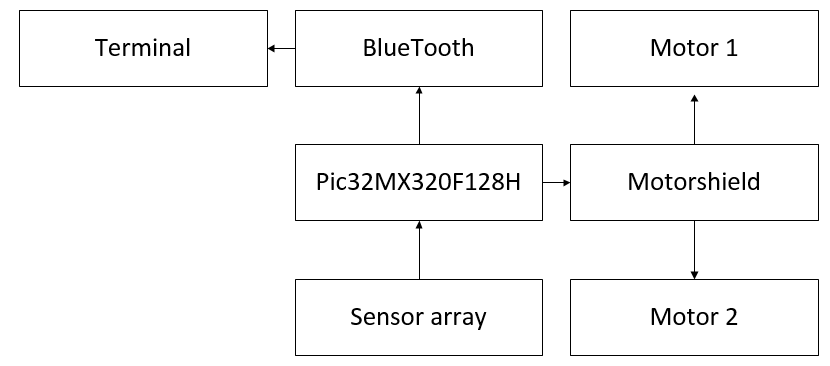
\includegraphics[width=.6\textwidth]{figures/hardwaredia.png}
	\caption{\text{Block diagram of the hardware.}}
	\label{Hardware diagram}
\end{figure}
    
\section{Selection of sensor}
\begin{table}[]
	\centering
	\label{Sensor table}
	\begin{tabular}{|l|l|l|}
		\hline
		Name                & QRE1113 Board & OPB704    \\ \hline
		Max sensor distance & 3mm           & 3.8mm     \\ \hline
		Forward current     & 50mA          & 40mA      \\ \hline
		Mounting            & On a PCB      & In casing \\ \hline
		Price               & 19.43DKK      & 42.55DKK  \\ \hline
	\end{tabular}
	\caption{Table showing the sensors in consideration}
\end{table}
The table shows a comparison of the two sensors that were taken into consideration for the project, this is to show the price difference and the specification differences from sensor to sensor. \emph{(fig 2.1)}

\subsection{The OPB704}
The OPB704 sensor ended up being selected for the robot over the popular QRE1113 sensor board. It has a higher sensor max distance (3.8mm\footnote{http://www.farnell.com/datasheets/1884910.pdf} compared to the QRE1113s 3mm) and it has the same functionality. It comes with a special casing, for which a special mounting unit was 3D-printed to accommodate an array of 7. This makes the mounting very solid and tightly fitted unto the robot, which ideally makes the sensor array more stable in case of an uneven test course.
\sidebyimg{figures/opb704.jpg}{The sensor OPB 704}{figures/sensorarray.jpg}{3D printed sensor array module}

\subsection{The QRE1113 board}
Another possible sensor selection would be the QRE1113\footnote{http://cdn.sparkfun.com/datasheets/Sensors/Proximity/QRE1113.pdf} board sensor. This sensor comes complete with mounting and the necessary printing and wiring. This makes working with the sensor fairly straightforward. Although this sensor is commonly used for line following robots, for this project the OPB704 sensor was chosen. This was done due to the accessibility and ease of mounting of the OPB 704 sensor.

\sidebyimg{figures/QRE.jpg}{QRE1113 Sensor on a breakout board}{figures/QREmount.jpg}{3D printed sensor array module withe the QRE1113}

\section{Analog-to-digital converter}
The purpose of the ADC is to convert the analog signal from the sensors, to digital data that can be managed by a computer. The sensors themselves cannot discern what signals are relevant and when to send these, the sensors just read anything they can see and send that signal. Analog signals can have a significant amount of noise since any received noise is interpreted as part of the signal.

\subsubsection{ADC diagram} 
\img{figures/ADCblock.png}{PIC32 ADC fuctional block diagram}{adcblockdiagram}{1}
\newpage
\subsubsection{This products usage of ADC}
The usage of the ADC in the system, is to measure the returning voltage from the OPB704 sensor. Both the OPB704 and the QRE1113 sensors are reflective phototransistors.
A reflective phototransistor consists of a infrared LED and a phototransistor.
The phototransitors output voltage is controlled by the amount of light from the LED that is being reflected off the given surface the sensor is pointed at, back to the phototransistor.
\img{figures/reflectivesensorworkings.png}{The difference in reflection on light and dark surfaces}{reflectivesensorworkings}{0.8}

\section{The chipKIT Uno32 board}
The main computing core is the chipKIT Uno32 board. The board was selected based on on previous experiences, and because it meets the set requirements - most importantly it has twelve analog imputs to handle our array of seven sensors; however the UCN board can only manage 6 sensors. This board utilizes the PIC32MX320F128 microcontroller, which features a 32-bit processing core running at 80MHz with 128KB of flash program memory and 16KB SRAM data memory\footnote{http://www.microchip.com/wwwproducts/en/PIC32MX320F128H}. 
This board has more than enough analog inputs which allows upwards of 12 sensors. Furthermore it allows for easier ADC conversions.
The board is compatible for use with MPLAB X IDE and the PICKit3 debugger.

\section{The motor shield - PKA03}
The motor shield was chosen because it is compatible with the Uno32 board, and fits perfectly within the scope of the project. It controls both motors and receives power from the 6.0 V battery pack mounted on the chassis itself. The motor shield is instrumental in providing motor controls to the product. To do this, it utilizes a specific electric circuit, called an H bridge.
\newpage
\subsection{The H bridge}
An H bridge is a circuit that allows a voltage to be applied across a load in either direction. The purpose of this in the case of this project is to enable controls of the two motors in a way so they can both function individually, and both drive forwards and backwards.\\

\section{The Bluetooth tranceiver}
The robot utilizes the BlueSMiRF Silver Bluetooth transceiver made by Sparkfun. Its function is to send data from the MCU (see the software section) to a C\# GUI run on a computer. This way, it is possible to monitor both the inputs the robot is receiving, as well as the logic behind the steering. It allows for any baudrate between 2400 to 115200\footnote{https://www.sparkfun.com/products/12577}. 

\input{contents/hardware/partconclusion.tex}
\chapter{Software section}
\subsection{Software diagram}
TBD Softwarediagram
\section{Description of the software structure and functionality}

The following section will introduce the software segment, based on our required specifications. The design will shown in the form of a flowchart.
TBD Softwarebeskrivelse og underafsnit

\subsection {Description of the PID controller} 
 
A PID controller continuously calculates an error value as the difference to a reference point and a measured process variable.\\
PID is an abbreviation for a proportional-integral-derivative controller, it is a control loop feedback mechanism. The controllers job is to minimize the error value for the given devices running time. In the case of this project the reference point is the line and the PID will power up the engines to steer accordingly to said reference point.
$$\mathrm{F}(t)=K_p{e(t)} + K_{i}\int_{0}^{t}{e(\tau)}\,{d\tau} + K_{d}\frac{de(t)}{dt}$$

\begin{figure}[h!]
  \centering
  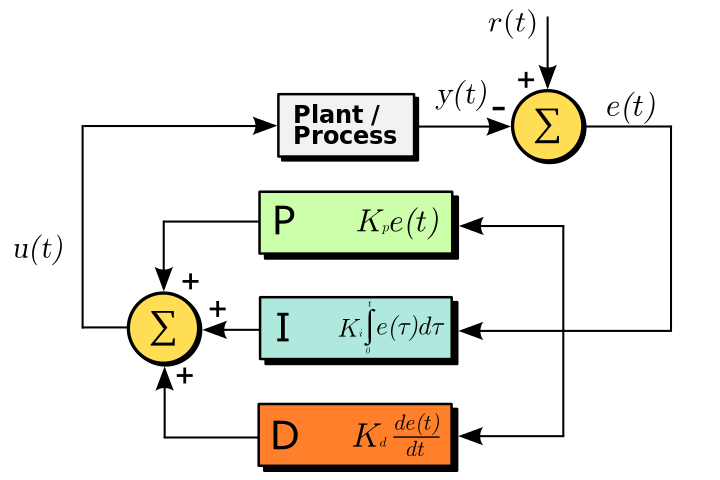
\includegraphics[width=0.5\textwidth]{figures/PID_block.png}
  
  \caption{Block diagram, showing the idea of PID controller. Credits: %https://en.wikipedia.org/wiki/PID_controller#/media/File:PID_en_updated_feedback.svg
  }
  \label{PID controller}
\end{figure}

\subsubsection {Proportional control(P)}

The proportional term creates an output value that is proportionally related to the current error value, this value can be tuned by multiplying the error by a constant $K_p$. A high proportional gain results in a large change in the output for a given change in the error. 


$$ P_{\mathrm{out}}=K_p\,{e(t)}$$  

If the proportional gain is too high, the system can become unstable. Contrarily, a small gain will result in the device adjusting too slowly, which decreases overall efficiency and in the case of this project, it will end up being detrimental to the steering accuracy.

\begin{figure}[h!]
  \centering
  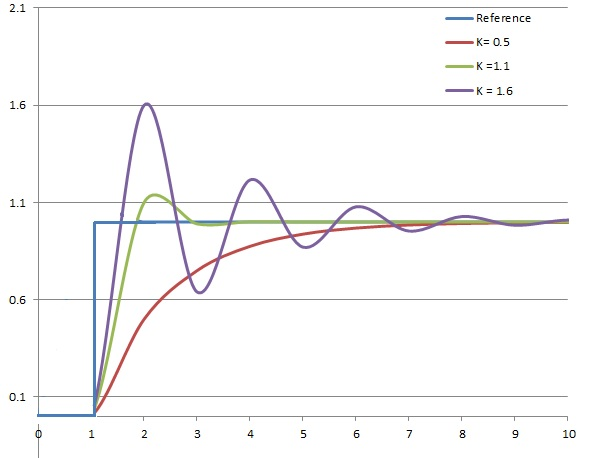
\includegraphics[width=0.5\textwidth]{figures/PIDP.jpg}
  
  \caption{$K_p$ with 3 values. ($K_i$, $K_d$ held constant) Credits: %https://en.wikipedia.org/wiki/PID_controller#/media/File:PID_varyingP.jpg
  }
  \label{PID controller}
\end{figure}


\subsubsection {Integral control(I)}



The integral controller is contributing proportionally to both the magnitude of the error and the duration of the error. \\
The integral in a PID controller is the sum of the instantaneous error over time and gives the accumulated offset that should have been corrected previously. \\ 

The controller output equals the accumulated error multiplied by the integral gain(Ki)\\
$$I_{\mathrm{out}}=K_{i}\int_{0}^{t}{e(\tau)}\,{d\tau}$$ 



The integral term accelerates the movement of the process towards the reference point.
Since the integral term correlates to accumulated errors from the past, it can cause the present value to overshoot the reference value.

\subsubsection {Derivative control(D)} 

The derivative of the process error is calculated by determining the slope of the error over time and multiplying this rate of change by the derivative gain $K_d$. The magnitude of the contribution of the derivative term to the overall control action is termed the derivative gain, $K_d$.
\begin{figure}[h!]
  \centering
  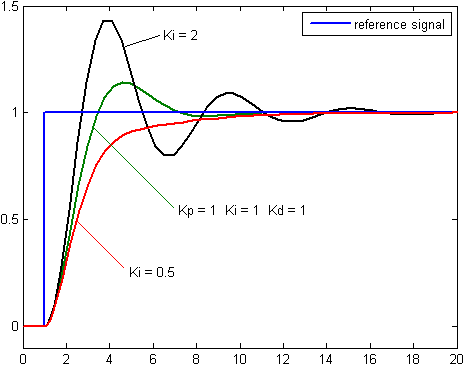
\includegraphics[width=0.5\textwidth]{figures/Change_with_Ki.png}
  
  \caption{$K_i$ shown with 3 values. Credits: %https://en.wikipedia.org/wiki/PID_controller#/media/File:Change_with_Ki.png
  }
  \label{PID controller}
\end{figure}

TBD (billede skal rettes ind til teksten)
The derivative term is given by:

$$D_{\mathrm{out}}=K_d\frac{de(t)}{dt}$$
The derivative action predicts system behaviour and utilizes this to improve the settling time and stability of the system.
An ideal derivative is not causal, so that implementations of PID controllers include an additional low pass filtering for the derivative term, to limit the high frequency gain and noise.

\begin{figure}[h!]
  \centering
  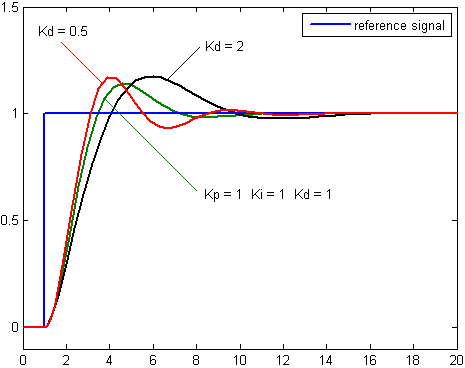
\includegraphics[width=0.5\textwidth]{figures/Change_with_Kd.png}
  
  \caption{$K_d$ shown with 3 values. Credits: %https://en.wikipedia.org/wiki/PID_controller#/media/File:Change_with_Kd.png
  }
  \label{PID controller}
\end{figure}



\subsubsection {Loop tuning} 

Tuning the loop is the term used to describe the adjustments of the PID’s control parameters (proportional band/gain, integral gain/reset, derivative gain/rate) to the optimal values for the given control scheme. \\ Stability is the first requirement; however systems can differ greatly, and different applications may have different requirements and these may even conflict with each other. For example, high speed and high accuracy often cancel each other out, because high speed may cause overshooting, while high accuracy is slow.\\ The ideal realistic behaviour is both as fast as possible, while also having minimum overshoot and oscillation. \\ 

Even though the process seems simple, with only three variables, it can be challenging to achieve, because it must satisfy the criteria despite being within the limitations of PID control. While adjusting the PID can seem conceptually intuitive, and while most PIDs may perform acceptably with default controls, they may very well also have an unsatisfactory performance.\\ This can generally be fixed through optimisation and tuning, either through computer simulations or manual testing. In our case, we used manual tuning of the numbers.

\subsubsection {Stability} 

If the parameters of the PID controller are set incorrectly the process input can become unstable.
This means the controllers output becomes divergent, this can be limited by saturation and mechanical breaking. \\

\subsubsection {Manual tuning} 

When a system must be online at all times a method for tuning is, to first set $K_i$ and $K_d$ values to zero. Increase $K_p$ until the loop output oscillates, setting $K_p$ at approximately half the value for a "quarter amplitude decay" type response.\\ %(TBD  kilde) (http://blog.opticontrols.com/archives/1066)
Then increase $K_i$ until any set off is corrected in sufficient time for the process. Adding too much $K_i$ will however cause an instability. 
Finally, increase $K_d$, if required at all, until the loop is acceptably quick to reach its reference after a load disturbance.
\\ 
A fast PID loop tuning process usually overshoots slightly to reach the reference point faster. 
In the case of systems that can't accept overshoot, an over-damped closed-loop system is best suited, which requires $K_p$ setting significantly less than half that of the $K_p$ setting that was causing the oscillation.

TBD (Vores fremgangsmåde med PID alt efter om "D" skal bruges)

% Please add the following required packages to your document preamble:
% \usepackage[table,xcdraw]{xcolor}
% If you use beamer only pass "xcolor=table" option, i.e. \documentclass[xcolor=table]{beamer}
\begin{table}[h]
\centering
\caption{Manual tuning}
\label{Table: Manual tuning}
\begin{tabular}{|l|l|l|l|l|l|}
\hline
\rowcolor[HTML]{C0C0C0} 
{\color[HTML]{000000} Parameter}                     & Rise time    & Overshoot & Settling time & Steady-state error  & Stability              \\ \hline
\cellcolor[HTML]{C0C0C0}{\color[HTML]{000000} $K_p$} & Decrease     & Increase  & Small change  & Decrease            & Degrade                \\ \hline
\cellcolor[HTML]{C0C0C0}{\color[HTML]{000000} $K_i$} & Decrease     & Increase  & Increase      & Eliminate           & Degrade                \\ \hline
\cellcolor[HTML]{C0C0C0}{\color[HTML]{000000} $K_d$} & Minor change & Decrease  & Decrease      & \begin{tabular}[c]{@{}l@{}}No effect\\ in theory\end{tabular} & \begin{tabular}[c]{@{}l@{}}Improves if\\ $K_d$ is small\end{tabular} \\ \hline
\end{tabular}
\end{table}

\subsubsection {Table 3.1 explained}

Table 3.1 gives an informative overview of what the different parameters does when tuned manually.

1. To decrease the rise time, use $K_p$ .\\
2. To reduce the overshoot and settling time, use $K_d$ .\\
3. To eliminate the steady-state error, use $K_i$ .\\
 
\input{contents/software/partconclusion.tex}
\chapter{Test}
\section{Testing round 1}

\subsection{Test description}
To make sure the product as a whole is working according to plan, testing must be done. First the components must be tested, this is done individually for each component to make sure there are no errors or fails when the product is built. The purpose of integration testing is to detect any inconsistencies between the software units that are integrated together. Testing is also done to watch the behavior of the product and tweak it.

\subsection{Unit Testing}
TBD testing af individuelle dele
Sensor
Motor
H-Bro
PWM

\subsection{Integration Testing}
TBD testing af interfacet og evt samarbejde mellem enkelte dele
Interface
PWM - motor

\subsection{System Testing}
TBD testing af systemet som helhed
Sensor - motor

\subsection{Acceptance Testing}
TBD testing af systemet som helhed. Acceptabel ydeevne?
Kan den klare banen? 
Evt. referer til video






\chapter{Conclusion}
The goal of this project was to make robot that could follow a black line by utilizing sensors and feedback control algorithms.
\\\\
During the project, a higher understanding of the workings of systems such as PID, ADC and PWM, and how they can be implemented in hardware and software was achieved. 
The solution was designed around the Magician Chassis and chipKIT Uno32 MCU Board. 
C code for the MCU has been made and implements the required systems: PID, ADC and PWM. Furthermore, an interface has been developed in C\#, that receives data through Bluetooth that the robot transmits through a BlueSMiRF Silver module.
\\\\
During the process, several problems occurred, most severe issues with the implementation of the PID algorithm. The algorithm was at first implemented wrong, adding in the derivative part instead of subtracting. This lead to a serious increase in time taken to tune the algorithm.\\
Furthermore, the first iteration of the robot included a homemade motor shield, which turned out to be faulty.\\
The product development ended in a success, resulting in a working robot that is able to navigate a line following track using the developed PID algorithm. 
\chapter{Appendices}
\section{Group collaboration agreement}
\subsection{Contact Information}
TBD contact info

\subsection{Workflow}
\begin{enumerate}
	\item[•]Every friday after 12:00 is expected work consisting of three hours.   
	\item[•]If you aren’t able of attending for scheduled study day. - Notice must be given to the project team. 
\end{enumerate}

\subsection{Milestones and goals}
TBD Milestones

\subsection{Deadline}
\begin{enumerate}
	\item[•]Hand in June 7th.
\end{enumerate}

\chapter{List of references}
PID: \\
\url{https://en.wikipedia.org/wiki/PID_controller#/media0/File:PID_en_updated_feedback.svg}\\

\url{https://en.wikipedia.org/wiki/PID_controller#Proportional_term}\\

\url{http://saba.kntu.ac.ir/eecd/pcl/download/PIDtutorial.pdf}\\

\url{http://blog.opticontrols.com/archives/1066}\\

\url{https://en.wikipedia.org/wiki/PID_controller#Steady-state_error}\\

\url{https://en.wikipedia.org/wiki/PID_controller#Integral_term}\\

\url{https://en.wikipedia.org/wiki/PID_controller#Derivative_term}\\

\url{https://en.wikipedia.org/wiki/PID_controller#Manual_tuning}\\

\url{https://en.wikipedia.org/wiki/PID_controller#Control_loop_basics}\\

\url{http://blog.opticontrols.com/archives/1066}

PWM:\\

\url{https://en.wikipedia.org/wiki/Pulse-width_modulation}\\

\newpage
\listoffigures
\addtocontents{lof}{~\hfill\textbf{Page}\par}
\newpage
\listoftables
\addtocontents{lot}{~\hfill\textbf{Page}\par}
\newpage
\printbibliography

\end{document}